\langsection[subsection]{Keeping Your Distance}{Сохраняйте дистанцию}

\begin{langblock}{0.425}
	\begin{eng}
	The best protection you can have is distance -- a ``cushion of space`` all around your motorcycle. If someone else makes a mistake, distance offers you:
	\begin{itemize}[noitemsep]
		\bfseries
		\item Time to react.
		\item Space to maneuver.
	\end{itemize}
	\end{eng}
	\begin{rus}
		Лучшая защита"--- это «пространственная подушка»\footnote{В русском языке разделяют <<запас спереди>> и <<по сторонам>> как <<Дистанция>> и <<Интервал>>. Чаще всего под ``cushion of space`` понимается именно интервал по сторонам. А дистанция или запас дистанции "--- это расстояние и/или время до того, что впереди} со всех сторон вашего мотоцикла. Если кто-то другой совершит ошибку, дистанция дает:
		\begin{itemize}[noitemsep]
			\bfseries
			\item Время для реакции
			\item Пространство для маневра
		\end{itemize}
\end{rus}
\end{langblock}



\langsection[subsubsection]{Lane Positions}{Положение в полосе}


\begin{figure}[htbp]
	\centering
	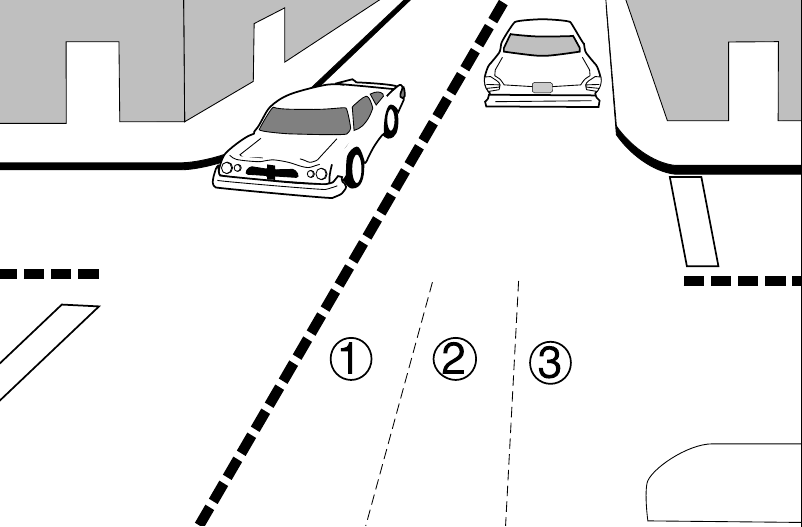
\includegraphics[width=0.75\textwidth, frame]{lane_pos}
	\caption{Lane positions}
	\label{fig:lane_pos1}
\end{figure}


\begin{langblock}{0.425}
	\begin{eng}
	In some ways the size of the motorcycle can work to your advantage. Each traffic lane gives a motorcycle three paths of travel, as indicated in the illustration.
	
	Your lane position should:
	\begin{itemize}[noitemsep]
		\item  Increase your ability to see and be
		seen.
		\item Avoid others' blind spots.
		\item Avoid surface hazards.
		\item Protect your lane from other
		drivers.
		\item Communicate your intentions.
		\item Avoid wind blast from other vehicles.
		\item Provide an escape route.
	\end{itemize}
	
	Select the appropriate path to maximize your space cushion and make yourself more easily seen by others on the road.
	
	In general, there is no single best position for riders to be seen and to maintain a space cushion around the motorcycle. No portion of the lane need be avoided -- including the center.
	
	Position yourself in the portion of the lane where you are most likely to be seen and you can maintain a space cushion around you. Change position as traffic situations change. Ride in path 2 or 3 if vehicles and other potential problems are on your left only. Remain in path 1 or 2 if hazards are on your right only. If vehicles are being operated on both sides of you, the center of the lane, path 2, is usually your best option.
	
	The oily strip in the center portion that collects drippings from cars is usually no more than two feet wide. Unless the road is wet, the average center strip permits adequate traction to ride on safely. You can operate to the left or right of the grease strip and still be within the center portion of the traffic lane. Avoid riding on big buildups of oil and grease usually found at busy intersections or toll booths.
	\end{eng}
	\begin{rus}
		В какой-то степени размеры мотоцикла это преимущество. Каждая полоса движения предоставляет мотоциклисту три траектории следования, как показано на иллюстрации.
		
		Выбранная позиция движения должна позволить:
		\begin{itemize}[noitemsep]
			\item Улучшить ваш обзор и самому быть более заметным.
			\item Избежать слепых зон других участников движения.
			\item Объезд опасных препятствий.
			\item Защищать вашу полосу от других водителей.
			\item Дать понять о ваши намерениях.
			\item Избежать воздушных порывов от других транспортных средств.
			\item Иметь путь отхода и маневра.
		\end{itemize}
		
		Выбирайте соответствующую полосу движения, чтобы максимально увеличить пространство вокруг вас и сделать себя более заметным для других участников дорожного движения.
		
		Как правило, не существует единственного оптимального положения на полосе, чтобы и быть заметным и поддерживать буфер безопасности вокруг себя. Не пренебрегайте никакой частью полосы  "--- включая центральную.
		
		Расположитесь в той части полосы, где вас с наибольшей вероятностью заметят и где вы сможете сохранять буфер безопасности вокруг себя. Меняйте позицию по мере изменения дорожных ситуаций. Двигайтесь в центральной или правой части, если транспортные средства и другие потенциальные опасности находятся только слева от вас. Оставайтесь в левой или средней зоне, если опасности находятся только справа. Если транспортные средства движутся по обеим сторонам от вас "--- лучшим вариантом будет центр полосы.
		
		Часть центральной полосы, которая накапливает подтеки масла от автомобилей, обычно имеет ширину не более двух футов. Если дорога не мокрая, центральная полоса обеспечивает достаточное сцепление для безопасного движения. Вы можете двигаться левее или правее от масляных следов, оставаясь при этом в центральной части. Избегайте езды по крупным скоплениям масла и смазки, которые обычно образуются на оживленных перекрестках или перед шлагбаумами пунктов оплаты.
\end{rus}
\end{langblock}





\langsection[subsubsection]{Following Another Vehicle}{Следование за другими авто}


\begin{langblock}{0.425}
	\begin{eng}
	``Following too closely`` is a major factor in crashes involving motorcyclists. In traffic, motorcycles need as much distance to stop as cars.  Normally, a minimum of four seconds distance should be maintained behind the vehicle ahead.
	
	To gauge your following distance:
	
	\begin{itemize}[noitemsep]
		\item Pick out a marker, such as a pavement marking or lamppost, on or near the road ahead.
		\item When the rear bumper of the vehicle ahead passes the marker, count off the seconds: ``one-thousand-one, one-thousand-two, one-thousand-three, one-thousand-four.``
		\item If you reach the marker before you reach ``four,`` you are following too closely.
	\end{itemize}
	
	%\emph{some emph text}, \textit{some it text}, \textsl{some sl text}, \textbf{some bf text}, \texttt{some tt text}, \textsc{some sc text}, \textsf{some sf text}, some palin text, 
	
	
	
	A four-second following distance leaves a minimum amount of space to stop or swerve if the driver ahead stops suddenly. It also permits a better view of potholes and other hazards in the road.
	
	A larger cushion of space is needed if your motorcycle will take longer than normal to stop. If the pavement is slippery, if you cannot see through the vehicle ahead, or if traffic is heavy and someone may squeeze in front of you, open up a five second or more following distance.
	
	Keep well behind the vehicle ahead even when you are stopped.  This will make it easier to get out of the way if someone bears down on you from behind. It will also give you a cushion of space if the vehicle ahead starts to back up for some reason.
	
	When behind a car, ride where the driver can see you in the rearview mirror. Riding in the center portion of the lane should put your image in the middle of the rearview mirror -- where a driver is most likely to see you.
	
	Riding at the far side of a lane may permit a driver to see you in a sideview mirror. But remember that most drivers don't look at their sideview mirrors nearly as often as they check the rearview mirror. If the traffic situation allows, the center portion of the lane is usually the best place for you to be seen by the drivers ahead and to prevent lane sharing by others.
	\end{eng}
	\begin{rus}
		Несоблюдение безопасной дистанции "--- основной фактор в ДТП с участием мотоциклистов. В условиях дорожного движения мотоциклам для остановки требуется такое же расстояние, как и автомобилям. Как правило, следует соблюдать дистанцию не менее четырех секунд до движущегося впереди транспортного средства.
		
		Для оценки дистанции в движении:
		\begin{itemize}[noitemsep]
			\item Выберите ориентир, например дорожную разметку или фонарный столб, на дороге впереди или рядом с ней.
			\item Когда задний бампер транспортного средства впереди проходит этот ориентир, начните считать секунды: «сто двадцать один, сто двадцать два, сто двадцать три, сто двадцать четыре».
			\item Если вы достигли ориентира до того, как досчитали до «четырех», вы едете слишком близко.
		\end{itemize}
		
		Если водитель впереди внезапно останавливается, дистанция в четыре секунды оставляет минимальное пространство для остановки или уклонения. Правильная дистанция это еще и лучший обзор выбоин и других препятствий на дороге.
		
		Большая дистанция необходима, если вашему мотоциклу требуется больше времени для остановки, чем обычно. Если дорожное покрытие скользкое, если вы не видите сквозь транспортное средство впереди или если движение интенсивное и кто-то может вклиниться перед вами "--- увеличьте дистанцию до пяти секунд и более.
		
		Даже когда вы остановились, держите дистанцию до транспортного средства впереди. Это даст возможность отъехать в строну, если кто-то наедет на вас сзади. Это также даст вам запас, если авто впереди по какой-то причине начнет откатываться назад.
		
		Когда вы едете позади автомобиля, расположитесь так, чтобы водитель мог видеть вас в зеркале заднего вида. Будучи в центральной части полосы ваше отражение будет в центре зеркала заднего вида "--- там, где водитель с наибольшей вероятностью вас увидит.
		
		Езда на крайних частях полосы должно дать водителю увидеть вас в боковых зеркалах. Однако помните, что большинство водителей не смотрят в них так часто как проверяют зеркало заднего вида. Если дорожная ситуация позволяет, то наилучший выбор "--- центральная часть. Чтобы вас видел водитель впереди и предотвратить заезд на вашу полосу других участников движения.
\end{rus}
\end{langblock}





\langsection[subsubsection]{Being Followed}{Если едут за вами}


\begin{langblock}{0.425}
	\begin{eng}
	Speeding up to lose someone following too closely only ends up with someone tailgating you at a higher speed.
	
	A better way to handle tailgaters is to get them in front of you. When someone is following too closely, change lanes and let them pass. If you can't do this, slow down and open up extra space ahead of you to allow room for both you and the tailgater to stop. This will also encourage them to pass. If they don't pass, you will have given yourself and the tailgater more time and space to react in case an emergency does develop ahead.
	\end{eng}
	\begin{rus}
		Ускорение с целью оторваться от водителя, следующего за вами слишком близко, приводит лишь к тому, что он продолжит висеть  «на хвосте», но уже на более высокой скорости.
		
		Правильнее будет пропустить его вперед. Если кто-то едет сзади слишком близко, перестройтесь в другую полосу и дайте ему возможность вас обогнать. Если сделать это невозможно, снизьте скорость. Если и это не побудит его совершить обгон, то на более низкой скорости у вас и у него будет больше времени и пространства для маневра на случай возникновения аварийной ситуации.
\end{rus}
\end{langblock}




\langsection[subsubsection]{Passing and Being Passed}{Обгон}


\begin{figure}[htbp]
	
	\begin{subfigure}{0.4\textwidth}
		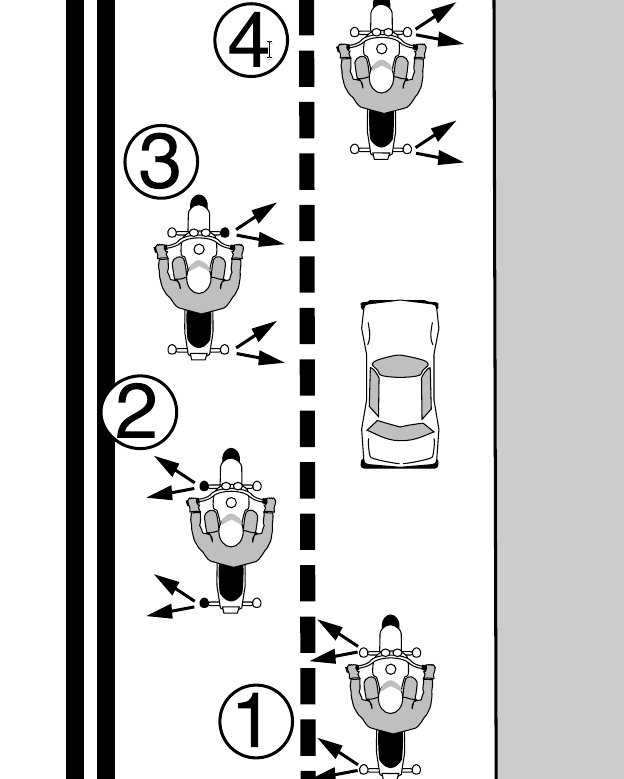
\includegraphics[width=0.95\textwidth, frame]{passing}
		\caption{Passing}
		\label{fig:passing1}
	\end{subfigure}	
	\hspace*{\fill}
	\begin{subfigure}{0.45\textwidth}
		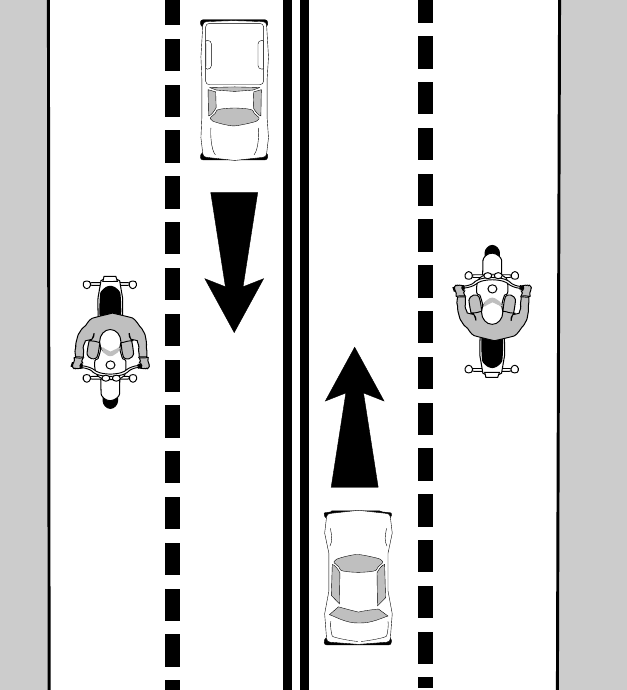
\includegraphics[width=0.95\textwidth, frame]{being_passed}
		\caption{Being passed}
		\label{fig:being_passed}
	\end{subfigure}
	\caption{Passing}
	\label{fig:passing}
\end{figure}


\begin{langblock}{0.425}
	\begin{eng}
	Passing and being passed by another vehicle is not much different than with a car. However, visibility is more critical. Be sure other drivers see you, and that you see potential hazards.
	\end{eng}
	\begin{rus}
		Обгон другого транспортного средства, а также ситуация, когда обгоняют вас, мало чем отличаются от аналогичных ситуаций при управлении автомобилем. Однако в данном случае особенно важна видимость. Убедитесь, что другие водители видят вас, а вы, в свою очередь, видите потенциальные опасности.
\end{rus}
\end{langblock}




\langsection[subsubsection]{Passing}{Когда обгоняете Вы}


\begin{langblock}{0.425}
	\begin{eng}
	\begin{enumerate}[noitemsep]
		\item Ride in the left portion of the lane at a safe following distance to increase your line of sight and make you more visible. Signal and check for oncoming traffic. Use your mirrors and turn your head\footnote{Headchecks --- is a law!\label{headchecksEN}} to look for traffic behind.
		
		\item When safe, move into the left lane and accelerate. Select a lane position that doesn't crowd the car you are passing and provides space to avoid hazards in your lane.
		
		\item Ride through the blind spot as quickly as possible.
		
		\item Signal again, and complete mirror and headchecks\footref{headchecksEN} before returning to your original lane and then cancel signal.
		
	\end{enumerate}
	{
		\bfseries
		Remember, passes must be completed within posted speed limits, and only where permitted.  Know your signs and road markings!
	}
	\end{eng}
	\begin{rus}
		\begin{enumerate}[noitemsep]
			\item Двигайтесь по левой части полосы, соблюдая безопасную дистанцию для лучшего обзора и большей заметности для других участников движения. Включите указатель поворота и проверьте наличие встречного транспорта. Посмотрите в зеркала заднего вида и обернитесь\footnote{Поворот головы "--- это не фигура речи: помимо зеркал необходимо физически повернуть голову, обернуться и посмотреть через плечо, это закон.\label{headchecksRU}}, чтобы проверить наличие транспорта позади себя.
			
			\item Когда это безопасно, перестройтесь на левую полосу и ускорьтесь. Выберите такое положение на полосе, которое не создает помех для обгоняемого автомобиля и оставляет пространство для маневра в случае возникновения опасной ситуации.
			
			\item Проедьте через «слепую зону» автомобиля как можно скорее.
			
			\item Снова включите указатель поворота, проверьте зеркала и обернитесь\footref{headchecksRU}, прежде чем вернуться на свою первоначальную полосу, после чего выключите указатель поворота\footnote{О да! Сколько из-за забытого поворотника может быть проблем. В авто поворотник отменяется сам, а на мото "--- нет.}.
			
		\end{enumerate}
		{
			\bfseries
			Помните: обгон должен выполняться в пределах установленного ограничения скорости и только там, где это разрешено. Следуйте указаниям дорожных знаков и разметки!
		}
\end{rus}
\end{langblock}




\langsection[subsubsection]{Being Passed}{Когда обгоняют Вас}


\begin{langblock}{0.425}
	\begin{eng}
	When you are being passed from behind or by an oncoming vehicle, stay in the center portion of your lane.  Riding any closer to them could put you in a hazardous situation. 
	
	Avoid being hit by:
	
	\begin{itemize}[noitemsep]
		\item The other vehicle -- A slight mistake by you or the passing driver could cause a sideswipe.
		\item Extended mirrors -- Some drivers forget that their mirrors hang out farther than their fenders.
		\item Objects thrown from windows -- Even if the driver knows you're there, a passenger may not see you and might toss something on you or the road ahead of you.	
		\item Blasts of wind from larger vehicles -- They can affect your control. You have more room for error if you are in the middle portion when hit by this blast than if you are on either side of the lane.
		
	\end{itemize}
	
	
	Do not move into the portion of the lane farthest from the passing vehicle. It might invite the other driver to cut back into your lane too early.
	\end{eng}
	\begin{rus}
		Когда мимо вас едет обгоняющий или встречный транспорт, держитесь центральной части своей полосы. Если вы будете находится ближе к проезжающему мимо вас транспортному средству, это может привести к возникновению опасной ситуации.
		
		Остерегайтесь следующего:
		
		\begin{itemize}[noitemsep]
			\item Другое транспортное средство "--- Небольшая ошибка с вашей или со стороны обгоняющего водителя может привести к боковому удару (скользящее столкновение).
			\item Выступающие зеркала заднего вида "--- Некоторые водители забывают, что их зеркала выступают за пределы кузова. Особенно ушастые внедорожники.
			\item Предметы, выброшенные из окна "--- Даже если водитель знает о вашем присутствии, вас может не заметить пассажир и выбросить что-либо из окна в вашу сторону или на дорогу перед вами.
			\item Порывы ветра от крупногабаритных транспортных средств "--- Они могут повлиять на управляемость вашего мотоцикла. Буквально переставлять мотоцикл в сторону на несколько футов. В средней части полосы у вас будет больше запаса для маневра, чем если бы вы находились у одного из ее краев.
		\end{itemize}
		
		
		Не отдаляйтесь в сторону от обгоняющего транспортного средства. Это может спровоцировать обгоняющего вернуться на вашу полосу слишком рано.
\end{rus}
\end{langblock}




\langsection[subsubsection]{Lane Sharing}{Движение по полосам}


\begin{langblock}{0.425}
	\begin{eng}
	Cars and motorcycles need a full lane to operate safely. Lane sharing is usually prohibited.
	
	Riding between rows of stopped or moving cars in the same lane can leave you vulnerable to the unexpected. A hand could come out of a window; a door could open; a car could turn suddenly. Discourage lane sharing by others. Keep a center- portion position whenever drivers might be tempted to squeeze by you.
	
	Drivers are most tempted to do this:
	\begin{itemize}[noitemsep]
		\item In heavy, bumper-to-bumper traffic.
		\item When they want to pass you.
		\item When you are preparing to turn at an intersection.
		\item When you are getting in an exit lane or leaving a highway.
	\end{itemize}
	\end{eng}
	\begin{rus}
		Автомобилям и мотоциклам для безопасного движения необходима полная ширина полосы. Совместное использование одной полосы несколькими транспортными средствами (бок о бок) обычно запрещено\footnote{Можно даже упростить до <<запрещено и все тут>>, но формально есть пара исключений}.
		
		Движение между рядами стоящих или движущихся автомобилей (lane splitting/filtering) в пределах одной полосы делает вас уязвимым перед неожиданностью. Из окна может высунуться рука; может внезапно открыться дверь; автомобиль может резко повернуть. Не позволяйте другим водителям пытаться пристроиться рядом с вами в одной полосе. Держитесь центральной части полосы всякий раз, когда у водителей может возникнуть соблазн протиснуться рядом с вами.\footnote{Соблазн есть и у мотоциклистов. В Пенсильвании ездить между машин в потоке (Lane-splitting) или просачиваться вперед на светофоре (Lane-filtering) запрещено. Lane-sharing разрешен только для двух мотоциклов, но не для машины и мотоцикла. См.  Title 75 Pa.C.S.A. Vehicles § 3523}
		
		Чаще всего у водителей возникает соблазн подвинуть вас на полосе:
		\begin{itemize}[noitemsep]
			\item В условиях плотного движения, когда автомобили едут «бампер в бампер».
			\item Когда они хотят вас обогнать.
			\item Когда вы готовитесь повернуть на перекрестке.
			\item Когда вы перестраиваетесь на полосу для съезда или покидаете шоссе.
		\end{itemize}
\end{rus}
\end{langblock}




\langsection[subsubsection]{Merging Cars}{Въезд и съезд на шоссе}


\begin{langblock}{0.425}
	\begin{eng}
	Drivers on an entrance ramp may not see you on the highway. Give them plenty of room. Change to another lane if one is open. If there is no room for a lane change, adjust speed to open up space for the merging driver.
	\end{eng}
	\begin{rus}
		Водители въезжающие на автомагистраль могут не заметить вас. Уступите, освободите им достаточно места. Перестройтесь в другую полосу, если она свободна. Если возможности перестроиться нет, скорректируйте скорость.
\end{rus}
\end{langblock}



\langsection[subsubsection]{Cars Alongside}{Езда параллельно с автомобилями}

\begin{figure}[htbp]
	\begin{subfigure}{0.45\textwidth}
		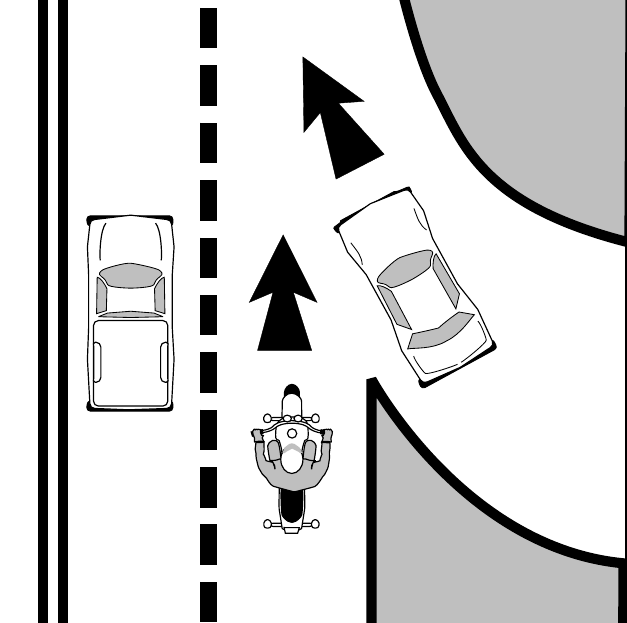
\includegraphics[width=0.95\textwidth, frame]{merging}
		\caption{Merging}
		\label{fig:meging}
	\end{subfigure}
	\hspace*{\fill}
	\begin{subfigure}{0.45\textwidth}
		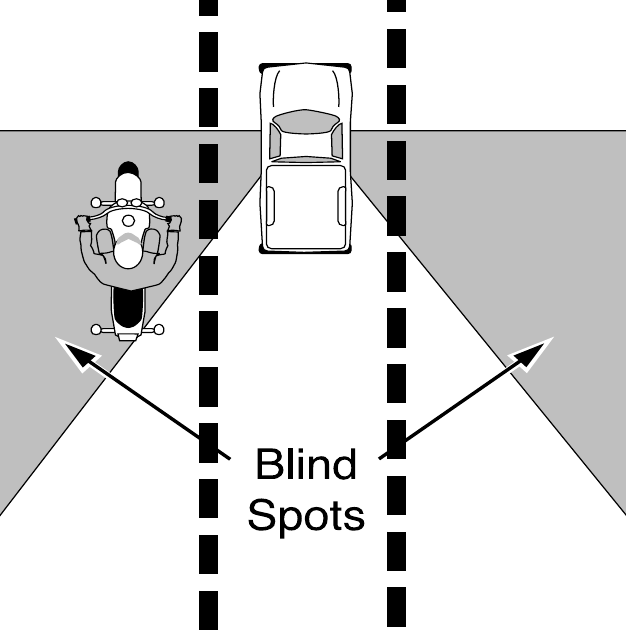
\includegraphics[width=0.95\textwidth, frame]{blind_spots}
		\caption{Blind spots}
		\label{fig:blind_spots}
	\end{subfigure}
	\caption{Merging cars and blind spots }
\end{figure}

\begin{langblock}{0.425}
	\begin{eng}
	Do not ride next to cars or trucks in other lanes if you do not have to.  You might be in the blind spot of a car in the next lane, which could switch into your lane without warning. Cars in the next lane also block your escape if you come upon danger in your own lane. Speed up or drop back to find a place clear of traffic on both sides.
	\end{eng}
	\begin{rus}
		Не двигайтесь параллельно с машинами или грузовиками без крайней необходимости. Вы можете быть в слепой зоне водителя на соседней полосе, который может перестроиться на вашу полосу без предупреждения. 
		Транспортные средства по бокам также блокируют пути маневра при возникновении опасности на вашей полосе. Ускорьтесь или от тормозитесь, чтобы занять участок, свободный от транспорта с обеих сторон.
\end{rus}
\end{langblock}























